\documentclass{ctexart}

\usepackage{ctex}

%各种需要用到的package
\usepackage{graphicx} % 插入图片用
\usepackage{amsmath} % 写定理环境用
\usepackage{amsthm} % 主要是方便用proof环境
\usepackage[linesnumbered, ruled, lined,boxed]{algorithm2e}[1] % 是写伪代码用

%把伪代码里面一些默认关键词改为中文
\renewcommand{\algorithmcfname}{算法}  %<---细节与重点
\SetKwInput{KwIn}{输入}  %<---细节与重点
\SetKwInput{KwOut}{输出}  %<---细节与重点

%声明定理类型
\newtheorem{definition}{定义}
\newtheorem{theorem}{定理}
\newtheorem{lemma}{引理}
\newtheorem{corollary}{推论}

%封面信息
\title{标题}
\author{张三 12345678}
\date{2023年5月10日}

\begin{document}

\maketitle
\begin{abstract}
	这是一个模板。
\end{abstract}

\newpage

\tableofcontents
\newpage

\section{介绍}
这是一个ctex模板,并且介绍了怎样使用这个模板。

\section{基本操作}
注册并登录overleaf账号。创建一个新的project,把模板当中的文件上传到project中。文件应该至少包含:main.tex,references.bib,图片。点左上角Menu,将编译器从pdfLaTeX改成XeLaTeX。点击右边的Recompile编译得到pdf。每次修改一部分内容之后都可以Recompile一下看看效果。

\textbf{注意} LaTeX正文当中,要空一行才算换行。
比如这里就没有换行。
以 及 空 格 是 无 效 的。

\section{公式和定理}
\subsection{公式}
想打公式,用(英文的)金钱符号括起来就行,比如$a^2+b^2=c^2$。公式里面的语法和普通文本不一样,具体可以在网上搜一下各种符号怎么打什么的。

\subsection{定理}
定理需要在前面声明类型。我已经声明了常用的几种。

用begin和end括起来的部分在LaTeX中称为环境。如下是一个theorem环境,可以用于陈述定理。
\begin{theorem}\label{thm:nodenum} %label是用于引用的
	在一棵结点数不小于$2$的树当中,叶子结点的个数$\geq$ 度数不小于$3$的结点数目$+2$。
\end{theorem}

\begin{proof}
	设叶子结点个数为$x_{1}$,度数为$2$结点个数为$x_{2}$,度数不小于$3$的结点数目为$x_{3^+}$。边的总数为$e$。

	由握手定理,
	\begin{align*}
		x_{1}+2x_{2}+3x_{3^+}\leq 2e
	\end{align*}

	由树的性质,
	\begin{align*}
		x_{1}+x_{2}+x_{3^+}=e+1
	\end{align*}

	上两式结合,易得$x_{1}\geq x_{3^+}+2$
\end{proof}

其它类型的定理环境也一样。
\begin{corollary}
	若图$G$是森林,则其中$1$度点总数不小于$3$度以上结点总数。
\end{corollary}

\section{图表和伪代码}
\subsection{图片}
插入图片示例如下:
\begin{figure}
	\centering
	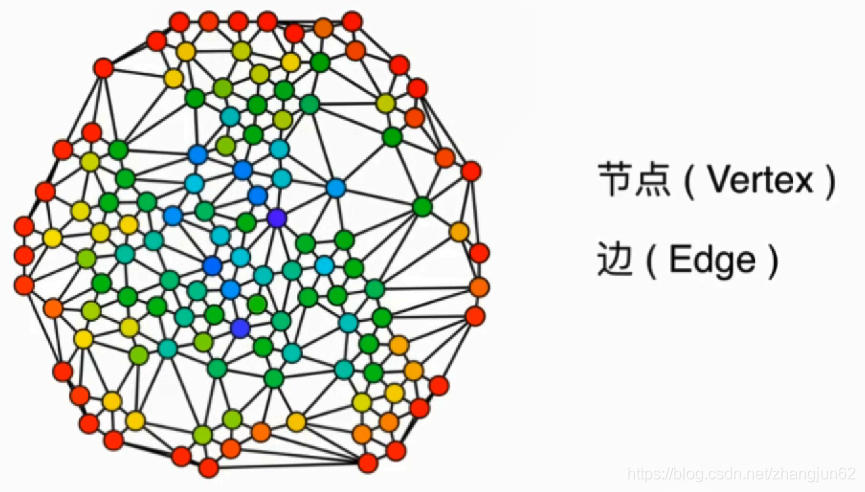
\includegraphics[scale=0.2]{example.png}
	\caption{简单无向图} \label{fig:gp} %这个\label可以用来引用
\end{figure}
可以调scale后面的参数来改变图片大小到合适。图\ref{fig:gp}是一个简单无向图的例子。

\subsection{表格}
表格示例如下:
\begin{table}[h!]
	\centering
	\begin{tabular}{c c c}
		\hline
		   & $1$度点  & $3$度以上点 \\
		\hline
		数量 & $10$   & $7$     \\
		比例 & $10\%$ & $7\%$   \\
		\hline
	\end{tabular}
	\caption{结点数目统计}
	\label{tab:nn}
\end{table}
表格也可以引用编号。比如表\ref{tab:nn}。

\subsection{伪代码}

伪代码示例如算法\ref{alg:rr}.

\begin{algorithm}[H]
	\caption{Reduction Rules}
	\label{alg:rr}
	\KwIn{图$G$}
	\KwOut{图$G'$}
	$G':= G,k':=k$.
	\While{$G'$中有$1$,$2$度点}{
		\If{$G'$中有$1$度点}{
			删除该$1$度点及其邻边,更新$G'$.
		}
		\If{$G'$中有$2$度点}{
			设该点为$v$,其邻居为$v_1,v_2$,令$G':=G'\setminus \{v,(v_1,v),(v,v_2)\}\cup \{(v_1,v_2)\}$.
		}
	}
	\textbf{RETURN($G'$)}.
\end{algorithm}

\section{引用参考文献}
所有的参考文献的完整信息都被存在bib文件里面。可以用\textbackslash cite命令在文中引用。比如:

根据文献\cite{cygan2015parameterized},定理\ref{thm:nodenum}可以被用于设计反馈集的参数算法。

bib文件里面的内容,可以通过dblp、google scholar等学术网站来获取。在这些网站上搜到对应的文章,可以直接找到对应的bibtex条目,复制进bib文件就可以。

\section{总结}
本文主要提供一个可以立刻上手来用的模板,不解释太多原理。想进一步学习LaTeX更高级的用法,同学们可以自己上网搜索,资料很多。

% 这是用来打印参考文献列表的
\bibliographystyle{plain}
\bibliography{references}

\end{document}
